\subsection{Opgaver}

\begin{enumerate}
	\item Lad $f\colon \R\to \R$ være givet ved
	\begin{align*}
	f(x)=\begin{cases}
	2x+3,& \textup{hvis } x\neq 1\\
	6,&\textup{ellers}.
	\end{cases}
	\end{align*}
	Bestem $\lim_{x\to 1}f(x)$, $f(1)$ og afgør om $f$ er kontinuert.
	
	
	\item Lad $f\colon \R\to \R$ være givet ved
	\begin{align*}
	f(x)=\begin{cases}
	2x^2-1,& \textup{hvis } x\neq 2\\
	7,&\textup{ellers}.
	\end{cases}
	\end{align*}
	Bestem $\lim_{x\to 2}f(x)$ og afgør om $f$ er kontinuert.

	
	
	\item Bestem de følgende grænseværdier
	\begin{align*}
	\lim_{x\to 3} x^2,&& \lim_{x\to 0} \frac{1}{x-1},&&\lim_{x\to -2} \frac{x^2-4}{x+2},&& \lim_{x\to 0} \frac{-2\frac{1}{x^3}-4\frac{1}{x^2}+12}{3\frac{1}{x^3}+\frac{1}{x}}
	\end{align*}
	


	
	
	\item Lad $f\colon \R\to \R$ være givet ved
	\begin{align*}
	f(x)=\begin{cases}
	\frac{1}{3}x+\frac{7}{6}, & \textup{hvis } x<-\frac{1}{2}\\
	-\frac{2}{3}x^2-\frac{1}{3}x+1,& \textup{hvis } x\geq -\frac{1}{2}.
	\end{cases}	
	\end{align*}
	Bestem grænsen $\lim_{x\to -\frac{1}{2}} f(x)$ såfremt den er veldefineret. 
	
	\item Lad funktionen $f\colon \R\to \R$ være givet ved
	\begin{align*}
	f(x)=\begin{cases}
	x^3+x-1,&\textup{hvis } x<1\\
	4x^4-2x^2+1,&\textup{hvis } x>1\\
	2,& \textup{ellers}.
	\end{cases}
	\end{align*}
	Hvad er $f(1)$? Er $f$ kontinuert i $1$.
	
	
	\item Bestem $a$ og $b$ så funktionen
	\begin{align*}
	f(x)=\begin{cases}
	ax,&\textup{hvis } x<1\\
	5,&\textup{hvis } x=1\\
	bx^2+x+1,& \textup{hvis }x>1
	\end{cases}
	\end{align*}
	er kontinuert i $1$.
	
	\item\label{it:lim2} Lad $f\colon \R\to \R$ være givet ved
	\begin{align*}
	f(x)=\begin{cases}
	\frac{x}{\abs{x}},&\textup{hvis } x\neq 0\\
	0 ,& \textup{ellers}.
	\end{cases}
	\end{align*}
	Bestem $ f(0) $, $ \lim_{x\to 0^+}f(x) $ og $\lim_{x\to 0^-}f(x)$. I hvilke punkter er $f$ kontinuert?
	
	\item Bestem grænserne
	\begin{align*}
	\lim_{x\to 2} \frac{x^2+4-4x}{x^2-4},&& \lim_{x\to -5} \frac{(x-1)(2x^2+14x+20)}{x^2+4x-5}
	\end{align*}
	
	\item Lad $f$ være givet som i Opgave~\ref{it:lim2} og lad $g(x)=-f(x)$. 
	\begin{enumerate}
		\item Bestem $ (f+g)(0) $, $ \lim_{x\to 0^+}(f+g)(x) $ og $\lim_{x\to 0^-}(f+g)(x)$. I hvilke punkter er $(f+g)$ kontinuert?
		\item Bestem $ (fg)(0) $, $ \lim_{x\to 0^+}(fg)(x) $ og $\lim_{x\to 0^-}(fg)(x)$. I hvilke punkter er $(fg)$ kontinuert?
	\end{enumerate}
	
	\item Funktionen $f\colon \R\to \R$ givet ved 
	\begin{align*}
	f(x)=\begin{cases}
	2x^2+x+1,&\textup{hvis } x\in [-a,a]\\
	x+2,&\textup{ellers}
	\end{cases}
	\end{align*}
	er plottet i \href{https://www.geogebra.org/m/mAmaHPC6}{GeoGebra}.
	\begin{enumerate}
		\item Bestem $a>0$ så $f$ er kontinuert.
		\item Er $f$ kontinuert når $a=0$?
	\end{enumerate}

	\item Bestem grænserne
	\begin{align*}
	\lim_{x\to 1} \frac{\ln x}{x},&& \lim_{x\to -2} (x^2-x)e^{x^2},&&  \lim_{x\to -1} x\ln(x+3).
	\end{align*}
	
	\item\label{it:lim1} I denne opgave bestemmes grænseværdien for funktionen $\frac{\sin x}{x}$ når $x$ går mod nul.
	\begin{enumerate}
		\item Figur~\ref{fig:lim1} viser vinklen $x\in [0,\frac{\pi}{2}[$ indtegnet i enhedscirklen. Brug figuren til at vise uligheden
		\begin{align*}
		\frac{1}{2}\sin x\leq \frac{1}{2}x\leq \frac{1}{2}\tan x.
		\end{align*}
		(Hint: Sammenlign arealet af det grå cirkeludsnit med arealet af $\Delta ACD$ og $\Delta ABD$ ).
		\item Omskriv uligheden fra (a) til 
		\begin{align*}
		\cos(x)\leq \frac{\sin x}{x}\leq 1.
		\end{align*}
		\item Brug at $\lim_{x\to 0} \cos(x)=1$ samt uligheden i (b) til at argumentere for at
		\begin{align*}
		\lim_{x\to 0}\frac{\sin x}{x}=1
		\end{align*}
	\end{enumerate}
	
	\begin{figure}
		\centering
		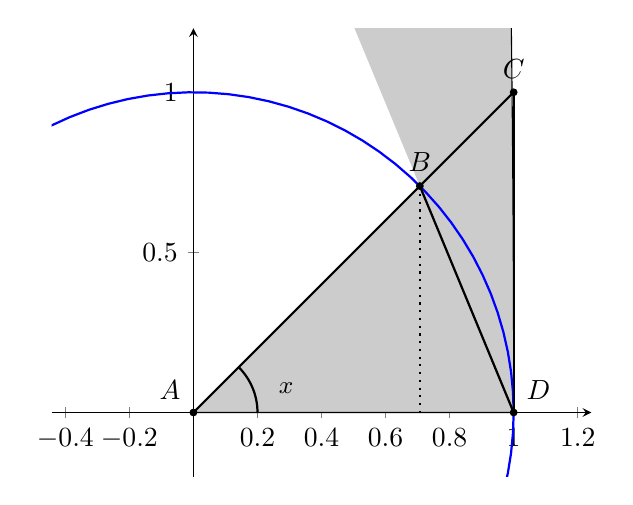
\begin{tikzpicture}
		\begin{axis}[xmin=-0.2,xmax=1,ymin=-0.2,ymax=1.2,axis x line=center,
		axis y line=center, axis equal]
				\pgfmathsetmacro\foo{sqrt(2)/2}
		\draw[fill=gray!40] (axis cs:0,0)--(axis cs:1,0)--(axis cs:\foo,\foo);		
		\draw[fill=gray!40] (axis cs:1,0)  arc[start angle=0, end angle=45,radius={transformdirectionx(1)}];

		\addplot[blue,domain=0:2*pi,thick, samples=100] ({cos(deg(x))},{sin(deg(x))});
		\addplot[domain=0:1,thick] {x};
		\addplot[domain=0:pi/4,thick,samples=100] ({0.2*cos(deg(x))},{0.2*sin(deg(x))}) node[label={[label distance=2pt]0:\small$x$},pos=0.5] {};
		\addplot[dotted,thick] coordinates {({sqrt(2)/2}, {sqrt(2)/2}) ({sqrt(2)/2}, 0)};
		\addplot[domain=sqrt(2)/2:1,thick] {{-x*sqrt(2)/(2-sqrt(2))+sqrt(2)/(2-sqrt(2))}};
		\addplot[thick] coordinates {(1,1) (1,0) };
		
		\node[fill, circle, inner sep=1pt] at (axis cs:0,0) [label=above left: $A$]{};
		\node[fill, circle, inner sep=1pt] at (axis cs:\foo,\foo) [label=above: $B$]{};
		\node[fill, circle, inner sep=1pt] at (axis cs:1,1) [label=above: $C$]{};
		\node[fill, circle, inner sep=1pt] at (axis cs:1,0) [label=above right: $D$]{};
		\end{axis}
		\end{tikzpicture}
		\caption{Opgave~\ref{it:lim1}}
		\label{fig:lim1}
	\end{figure}

	\item\label{it:lim3} Vis at 
	\begin{align*}
	\lim_{x\to 0}\frac{\cos (x)-1}{x}=0.
	\end{align*} 
	(Hint: Bruge Opgave~\ref{it:lim1}, identiteten
	\begin{align*}
	\frac{\cos (x)-1}{x}=\frac{\sin^2 x}{x(1+\cos x)}= \frac{\sin x}{x}\frac{\sin x}{1+\cos x}
	\end{align*}
	og produktreglen for grænser.)
	
	\item \label{it:lim4} Brug Opgave~\ref{it:lim1} del (b) til at vise at
	\begin{align*}
	\frac{\cos(x)-1}{x}\leq \frac{\sin(x)-x}{x^2}\leq 0.
	\end{align*}
	Argumenter vha. Opgave~\ref{it:lim3} for at 
	\begin{align*}
	\lim_{x\to 0}\frac{\sin(x)-x}{x^2}=0.
	\end{align*}
	
	\item\label{it:lim5} Vis at 
	\begin{align*}
	\lim_{x\to 0}\frac{\cos (x)-1}{x^2}=\frac{1}{2}.
	\end{align*} 
	(Hint: Bruge Opgave~\ref{it:lim1}, identiteten
	\begin{align*}
	\frac{\cos (x)-1}{x^2}=\frac{\sin^2 x}{x^2(1+\cos x)}= \Big(\frac{\sin x}{x}\Big)^2\frac{1}{1+\cos x}
	\end{align*}
	og produktreglen for grænser.)	
		
	
\end{enumerate}